\section{Educational Games for Private Consumers}
\label{sec:privateconsumers}
Many companies create educational games for children to learn math, languages and other basic school topics.
Most of these games are targeted towards younger children, who are about to start school or are in elementary school.
A company like Krea Games \cite{kreagames} creates multiple series for differently aged children.
These games are mostly available for PC, with a small subset also being available for Android and iOS devices.
In the following subsection, we will examine some of the best selling educational games for private consumers, explain why we feel they are good games and how features of these games can be used in combination with our product.

\subsection{Best Selling Educational Games}
One of the most popular educational games is The Oregon Trail, released first in 1982 with more than 65 million copies sold worldwide since.\cite{oregontrail} The game was originally released to teach children in American schools about how pioneers lived in the 19th century, but was also released to the general public as a standalone game for the home PC. The Oregon Trail was one of the first video games ever used in the United States for educational purposes, which has added  significantly to its popularity and cult status.

The objective of the game is to help a family/group of American pioneers follow the Oregon Trail and make sure, that they survive their endeavor to finally settle down in Oregon. The game teaches children the history of the Oregon Trail without sacrificing the gameplay experience, and thus the game is considered a good game even without the educational aspect.\newline

\todo{New material for Martin} As with Global Conflict, the game includes a sense of realism. It is possible to die from various diseases, cattle being stolen, food rations getting low etc. It seems, that focusing making the game seem realistic is part of the engaging nature of both games. We feel, that both games do not impress in terms of graphics. We therefore feel, that it is less important how the game looks graphically and more important to focus on creating a situation that the players wants to interact with and learn more about and that is realistic.\newline

Other popular educational games include:
\begin{itemize}
	\item[Where in the World Is Carmen Sandiego?] A game released in 1985, that teaches geography. The game was popular enough to spawn several sequels released as late as in 1998 and the first version of the game was released in 2011 as a Facebook version.\cite{carmensandiego}
	\item[Lemonade Stand] A game created by Bob Jamison and released in 1973, which teach the player about economics.\cite{lemonadestand}
\end{itemize}

\paragraph{Where in the World Is Carmen Sandiego?} is centered around the detective Carmen, who travels around the world in order to capture criminals. Learning geography is an essential part of the game, since the player has to follow clues to where in the world a thief they need to catch has gone. Later games in the series taught different subjects such as history or math.\todo{What aspect of the game can be included in our game?}

\todo{New material for Martin}\paragraph{Lemonade Stand} is a game, where the players plays as a child whom has a lemonade stand.
The player makes choices regarding the cost of the lemonade, money spent on advertising and how many glasses of lemonade to make, thereby teaching basic economics in a fun and relatable way for children. \textbf{Eventhough lemonade stands are not very common in Denmark, the aspect of making the game relatable to the consumer seems to be an important factor.} Maybe this is one of the aspects that has made the game so popular, since several remakes of the game has been released throughout the years, which are still very popular.\newline

Judging by these games, it is possible to create a game that is both engaging and educational, while not making it too obvious that the game is educational. Thus the player does not feel like he is doing homework while playing the game. \todo{New material for Martin}We have seen, that the aspects reality, realism and relatability may be to blame for part of the success of the above mentioned games and that if possible, these aspects should be included in our final product.

\subsection{Browser-based Educational Games}
Most educational games, that can be accessed from a browser on the home PC, are flash games on websites. Some of these claim to be approved by teachers for educational purposes.
Many if the games that we have found are heavily inspired by classic games, such as a Pac-Man like game called Math Man, where the player has to play Pac-Man while doing math problems to win.\cite{mathman}
Grand Prix Multiplication is another example, which is a multiplayer racing game, where the player has to do multiplication to make the car drive faster in order to win.\cite{grandprix}\newline

Brower-based games are good in terms of availability, since most households has a PC and in many cases, each family members has his/her own PC with assess to the internet. Most brower-based games are also free-to-play, which also increase their availability. However, our overall impression of the browser-based educational games is, that they are very explicit in their teaching method. This can be a good thing if the game is primarily used in schools, where the purpose is to teach new material. However, the explicit nature of these games can make them seem like homework and keep the children from playing the games when they are at home. We found, that in general the games we look at neglected the entertainment and engaging aspect of video games. It is important to avoid explicit teaching in our final product.\newline

%The prices of educational games varies from platform to platform. 
%Games on tablets ranges from free to about DKK 30, where both platforms are possible subjects to a form of micro transaction system.
%Downloadable PC games cost from DKK 30 to around DKK 100.
%Prices on educational games are as such significantly lower than prices of regular games, which usually has a release cost of between DKK 300-400 for PC games.\todo{Maybe missing source}

\subsection{Teaching Programming with Games}
We have not been able to find many games that try to teach programming fundamentals. Carnage Heart for the original PlayStation is one of the few that exist. In the game, the player has to create a robot that has to fight other robots in a war. However, the robot cannot be controlled directly, instead the player has to program its behavior using a grid of icons, as seen on \autoref{fig:carnageheartsoftware}.

\begin{figure}[h]
  \centering
    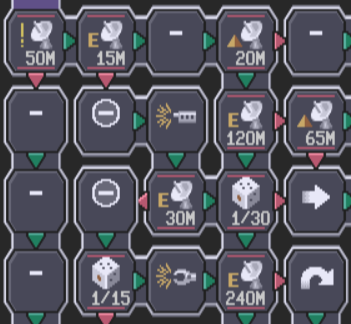
\includegraphics[width=0.5\textwidth]{img/CarnageHeartSoftware.png}
  \caption{Screenshot of the programming interface in Carnage Heart.\cite{carnageheartsoftware}}
  \label{fig:carnageheartsoftware}
\end{figure}

Carnage Heart teaches only basic programming constructs, but do not present them as such. Instead the player is presented with a set of rules, which are much like the rules of programming, and are told to create what is basically an AI for the robot.\\

Another example of a game trying to teach programming is CodeCombat. \cite{codecombat} CodeCombat is a browser-based game, that tries to teach JavaScript programming by making the player write code to play an RPG. The player plays as a wizard, and the programming is represented as magic spells in the game. The player is programming an AI for a knight, that has to fight a variety of monsters. Control of the knight includes movement and attack as well as conditions such as attack if the enemy is in range.
Although CodeCombat is a game, it is very explicit in its teaching.\todo{Why?} Tools such as Codecademy provide the same kind of programming guides as CodeCombat, but without the gaming aspect.\cite{codecademy}\\

Microsoft has released a game for teaching children programming called Kodu Game Lab. \cite{kodu} Kodu Game Lab is a free game on the PC and can be bought for $\$4.99$ on the Xbox 360 marketplace. This means, that the game is available to most children. In the game, the player starts with a small world, a square of grass. The player can then add objects and program them to do what the player wants. It is possible to make an object react to other objects, e.g. eat them. The programming interface, see figure \autoref{fig:kodu}, in Kodu Game Lab is very simple, and visually illustrates what will happen. 

\begin{figure}[h]
  \centering
    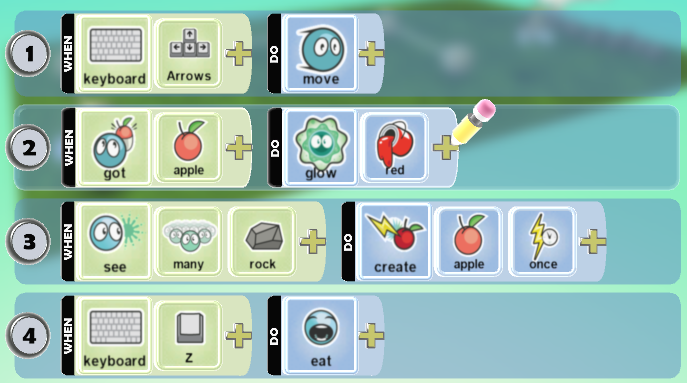
\includegraphics[width=\textwidth]{img/kodu.png}
  \caption{Screenshot of the programming interface in Kodu Game Lab.}
  \label{fig:kodu}
\end{figure}\todo{source}

The way Carnage Heart and Kodu Game Lab approach teaching basic programming constructs is very relevant to our project, and could be a source of inspiration when we need to design our own game.